\documentclass[12pt,a4paper]{article}

% ── Paquetes ──
\usepackage[utf8]{inputenc}
\usepackage[spanish]{babel}
\usepackage[left=2.5cm,right=2.5cm,top=2.5cm,bottom=3cm]{geometry}
\usepackage{float}
\usepackage{graphicx}
\usepackage{enumitem}
\usepackage{booktabs}
\usepackage{amsmath,amssymb}
\usepackage[hidelinks]{hyperref}
\usepackage{parskip}
\usepackage{caption}
\usepackage{subcaption}
\usepackage{listings}
\usepackage{xcolor}
\usepackage{fancyhdr}
\usepackage{titlesec}

\setlength{\parindent}{1.27cm}

% ── Estilo de código ──
\definecolor{codebg}{HTML}{F5F5F5}
\definecolor{codeframe}{HTML}{CCCCCC}
\definecolor{codecomment}{HTML}{6A9955}
\definecolor{codestring}{HTML}{CE9178}
\definecolor{codekeyword}{HTML}{569CD6}

\lstset{
  language=Python,
  basicstyle=\ttfamily\small,
  backgroundcolor=\color{codebg},
  frame=single,
  rulecolor=\color{codeframe},
  keywordstyle=\color{codekeyword}\bfseries,
  commentstyle=\color{codecomment}\itshape,
  stringstyle=\color{codestring},
  showstringspaces=false,
  breaklines=true,
  numbers=left,
  numberstyle=\tiny\color{gray},
  numbersep=8pt,
  tabsize=4,
  captionpos=b,
  aboveskip=1em,
  belowskip=1em,
}

% ── Encabezados y pies ──
\pagestyle{fancy}
\fancyhf{}
\fancyhead[L]{\small\textit{Péndulo Simple — Visión Computacional y FFT}}
\fancyhead[R]{\small\textit{UTB}}
\fancyfoot[C]{\thepage}
\renewcommand{\headrulewidth}{0.4pt}

% ── Formato de secciones ──
\titleformat{\section}{\Large\bfseries}{\thesection.}{0.5em}{}
\titleformat{\subsection}{\large\bfseries}{\thesubsection.}{0.5em}{}
\titleformat{\subsubsection}{\normalsize\bfseries}{\thesubsubsection.}{0.5em}{}

\begin{document}

% ════════════════════════════════════════════════════════════════
% PORTADA
% ════════════════════════════════════════════════════════════════
\begin{titlepage}
	\centering
	
\includegraphics[width=0.50\textwidth]{../../resources/logos/Nuevo-logo-UTB-1.png}\par\vspace{0.5cm}
	{\scshape\LARGE\textbf{Universidad Tecnológica de Bolívar} \par}
	\vspace{1.5cm}
	\rule{\linewidth}{0.2mm}\\[0.4cm]
	{\huge\bfseries Estimación del periodo de oscilación de un péndulo simple \par}
	\rule{\linewidth}{0.2mm}\\[1.0cm]
	\vspace{0.5cm}

	{\large\textbf{Actividad 2 — Segundo corte} \par}
	\vspace{0.3cm}
	{\large Sensado y Modelado de Sistemas Físicos \par}
	\vspace{1.5cm}

	\centering{\emph{\textbf{Estudiantes:}}\\
		German De Armas Castaño \\
		Angel Vega Rodriguez \\
		Michael Taboada Naranjo\\}

	\vspace{1cm}
	\centering{\emph{\textbf{Profesor:}}\\
		David Sierra Porta\\}

	\vfill
	{\large \today\par}
\end{titlepage}

\tableofcontents
\newpage

% ════════════════════════════════════════════════════════════════
% 1. INTRODUCCIÓN
% ════════════════════════════════════════════════════════════════
\section{Introducción}

El presente reporte documenta el diseño, implementación y validación de un sistema automatizado para la estimación del \textbf{periodo de oscilación} de un péndulo simple a partir del procesamiento de video. El proyecto se desarrolló en dos fases:

\begin{enumerate}[label=\textbf{\arabic*.}]
    \item \textbf{Fase de exploración y prototipado} --- implementada en el notebook: \\ \texttt{pendulum\_analyzer.ipynb}. Aquí se diseñaron y validaron los algoritmos de visión computacional, reconstrucción angular, detección de picos, análisis espectral (FFT) y ajuste de amortiguamiento.
    \item \textbf{Fase de productización} — los hallazgos del notebook se encapsularon en una aplicación web interactiva (React + FastAPI) integrada al ecosistema \textbf{Bento Launcher}.
\end{enumerate}

La narrativa del documento sigue el flujo natural del trabajo: fundamentos teóricos, implementación detallada en el notebook, y finalmente la materialización en la aplicación web.

\subsection{Planteamiento del problema}

El péndulo simple es uno de los sistemas dinámicos más estudiados en física. Su periodo de oscilación depende de la longitud de la cuerda y de la aceleración gravitatoria, lo que lo convierte en un instrumento clásico para estimar $g$. Sin embargo, medir el periodo manualmente presenta limitaciones:

\begin{itemize}
    \item La \textbf{latencia de reacción humana} al accionar un cronómetro introduce errores del orden de $\pm 200$ ms.
    \item Para ángulos grandes ($\theta_0 > 15^{\circ}$), la aproximación lineal $\sin\theta \approx \theta$ deja de ser válida, y el periodo real difiere del teórico simple.
    \item El \textbf{amortiguamiento} por fricción causa que la amplitud decaiga con el tiempo, dificultando la medición de periodos consistentes.
\end{itemize}

Un sistema de visión computacional combinado con análisis espectral permite superar estas limitaciones, extrayendo la dinámica completa del sistema a partir de un video.

\subsection{Objetivos}

\begin{enumerate}[label=\textbf{\arabic*.}]
    \item Implementar un algoritmo de segmentación por color (HSV) para rastrear la masa del péndulo frame a frame.
    \item Reconstruir la trayectoria angular $\theta(t)$ a partir de las coordenadas del centroide y la posición conocida del pivote.
    \item Estimar el periodo de oscilación mediante tres métodos independientes: cruces por cero, detección de picos y Transformada Rápida de Fourier (FFT).
    \item Comparar los resultados experimentales con los valores teóricos (aproximación lineal y corrección de Borda).
    \item Analizar el amortiguamiento del sistema mediante ajuste exponencial de la envolvente de amplitudes.
    \item Encapsular el pipeline en una aplicación web desplegable desde el Bento Launcher.
\end{enumerate}

\subsection{Parámetros de la simulación}

El video analizado fue generado mediante una simulación numérica con los siguientes parámetros conocidos:

\begin{table}[H]
    \centering
    \begin{tabular}{lcc}
        \toprule
        \textbf{Parámetro} & \textbf{Símbolo} & \textbf{Valor} \\
        \midrule
        Aceleración gravitatoria & $g$ & 9.81 m/s$^2$ \\
        Longitud de la cuerda & $L$ & 1.0 m \\
        Ángulo inicial & $\theta_0$ & $45^{\circ}$ \\
        Coeficiente de fricción & $\mu$ & 0.05 \\
        Frames por segundo & FPS & 30 \\
        Escala espacial & --- & 400 px/m \\
        \bottomrule
    \end{tabular}
    \caption{Parámetros conocidos de la simulación del péndulo.}
    \label{tab:params}
\end{table}

% ════════════════════════════════════════════════════════════════
% 2. FUNDAMENTOS TEÓRICOS
% ════════════════════════════════════════════════════════════════
\section{Fundamentos Teóricos}

\subsection{Ecuación de movimiento del péndulo simple}

La ecuación diferencial que gobierna el movimiento de un péndulo simple ideal (sin fricción) es:

\begin{equation}
    \ddot{\theta} + \frac{g}{L}\sin\theta = 0
\end{equation}

Para oscilaciones de pequeña amplitud ($\theta \ll 1$ rad), se aplica la aproximación $\sin\theta \approx \theta$, obteniendo un oscilador armónico simple con periodo:

\begin{equation}
    \label{eq:T-lineal}
    T_{\text{lineal}} = 2\pi\sqrt{\frac{L}{g}}
\end{equation}

\subsection{Corrección para ángulos grandes (Borda)}

Para ángulos iniciales grandes, el periodo real es mayor que el predicho por la ecuación~\eqref{eq:T-lineal}. La corrección de Borda expande el periodo exacto en serie de potencias del ángulo inicial:

\begin{equation}
    \label{eq:T-borda}
    T_{\text{Borda}} \approx T_{\text{lineal}} \left(1 + \frac{1}{16}\theta_0^2 + \frac{11}{3072}\theta_0^4 + \cdots\right)
\end{equation}

Para $\theta_0 = 45^{\circ} \approx 0.785$ rad, la corrección es del orden del 4--5\%, lo que la hace significativa y necesaria para una comparación rigurosa.

\subsection{Péndulo amortiguado}

Al incluir fricción proporcional a la velocidad angular, la ecuación de movimiento se modifica:

\begin{equation}
    \ddot{\theta} + 2\gamma\dot{\theta} + \frac{g}{L}\sin\theta = 0
\end{equation}

donde $\gamma$ es el coeficiente de amortiguamiento. La amplitud de las oscilaciones decae exponencialmente:

\begin{equation}
    \label{eq:damping}
    A(t) = A_0\, e^{-\gamma t}
\end{equation}

La constante de tiempo $\tau = 1/\gamma$ indica el tiempo en que la amplitud se reduce a $1/e$ de su valor inicial.

\subsection{Reconstrucción angular desde coordenadas de píxeles}

Conocida la posición del pivote $(x_p, y_p)$ y la posición de la masa $(x_m, y_m)$ en cada frame, el ángulo respecto a la vertical se calcula como:

\begin{equation}
    \label{eq:theta}
    \theta = \arctan\!\left(\frac{x_m - x_p}{y_m - y_p}\right)
\end{equation}

donde se utiliza \texttt{arctan2} para preservar el signo y el cuadrante correcto.

\subsection{Transformada Rápida de Fourier (FFT)}

La FFT descompone una señal discreta $x[n]$ de $N$ muestras en sus componentes de frecuencia:

\begin{equation}
    X[k] = \sum_{n=0}^{N-1} x[n]\, e^{-i 2\pi k n / N}, \qquad k = 0, 1, \ldots, N-1
\end{equation}

El \textbf{espectro de potencia} $|X[k]|^2$ revela las frecuencias dominantes de la señal. La frecuencia fundamental $f_0$ corresponde al pico de mayor magnitud, y el periodo se obtiene como $T = 1/f_0$.

Para reducir el \textbf{leakage espectral} (dispersión de energía causada por la truncación de la señal), se aplica una \textbf{ventana de Hanning} antes de la FFT:

\begin{equation}
    w[n] = \frac{1}{2}\left(1 - \cos\!\left(\frac{2\pi n}{N-1}\right)\right)
\end{equation}

\subsection{Reconstrucción por series de Fourier}

La señal original puede reconstruirse utilizando los $K$ armónicos más significativos:

\begin{equation}
    \theta_{\text{rec}}(t) = \frac{a_0}{2} + \sum_{k=1}^{K} \left[ a_k \cos(2\pi f_k t) + b_k \sin(2\pi f_k t) \right]
\end{equation}

Esto permite evaluar cuántos términos son necesarios para capturar la dinámica del sistema y cuantificar el error de reconstrucción mediante el RMSE.

% ════════════════════════════════════════════════════════════════
% 3. IMPLEMENTACIÓN EN EL NOTEBOOK
% ════════════════════════════════════════════════════════════════
\section{Implementación en el Notebook}

El notebook \texttt{pendulum\_analyzer.ipynb} estructura el análisis en ocho módulos secuenciales. A continuación se detalla cada uno.

\subsection{Módulo 1: Detección de la masa (\texttt{detect\_pendulum\_mass})}

La función de detección sigue el mismo pipeline validado en el proyecto del coeficiente de restitución:

\begin{enumerate}
    \item Conversión BGR $\rightarrow$ HSV.
    \item Umbralizado por rango: $H \in [0, 15]$, $S \in [80, 255]$, $V \in [80, 255]$ (masa roja).
    \item Limpieza morfológica (apertura + cierre, kernel elíptico $5 \times 5$).
    \item Búsqueda de contornos y selección del mayor.
    \item Cálculo del centroide $(c_x, c_y)$ mediante momentos espaciales.
\end{enumerate}

\begin{lstlisting}[caption={Función de detección de la masa del péndulo.}]
def detect_pendulum_mass(frame, lower_hsv, upper_hsv, min_area=100):
    hsv = cv2.cvtColor(frame, cv2.COLOR_BGR2HSV)
    mask = cv2.inRange(hsv, lower_hsv, upper_hsv)

    kernel = cv2.getStructuringElement(cv2.MORPH_ELLIPSE, (5, 5))
    mask = cv2.morphologyEx(mask, cv2.MORPH_OPEN, kernel)
    mask = cv2.morphologyEx(mask, cv2.MORPH_CLOSE, kernel)

    contours, _ = cv2.findContours(
        mask, cv2.RETR_EXTERNAL, cv2.CHAIN_APPROX_SIMPLE)
    if not contours:
        return None

    largest = max(contours, key=cv2.contourArea)
    if cv2.contourArea(largest) < min_area:
        return None

    M = cv2.moments(largest)
    if M["m00"] == 0:
        return None

    cx = int(M["m10"] / M["m00"])
    cy = int(M["m01"] / M["m00"])
    return (cx, cy)
\end{lstlisting}

\subsection{Módulo 2: Tracking y extracción de series temporales}

El video se recorre frame a frame. Para cada detección exitosa se registra el instante temporal $t = \text{frame\_idx} / \text{FPS}$ y las coordenadas $(x, y)$ del centroide. El resultado son tres arrays NumPy: \texttt{times}, \texttt{x\_positions} y \texttt{y\_positions}.

\subsection{Módulo 3: Reconstrucción de la trayectoria angular}

Con las coordenadas del pivote conocidas (centro superior del lienzo, $(400, 100)$ px), se aplica la ecuación~\eqref{eq:theta} para obtener $\theta(t)$ en radianes.

\begin{figure}[H]
    \centering
    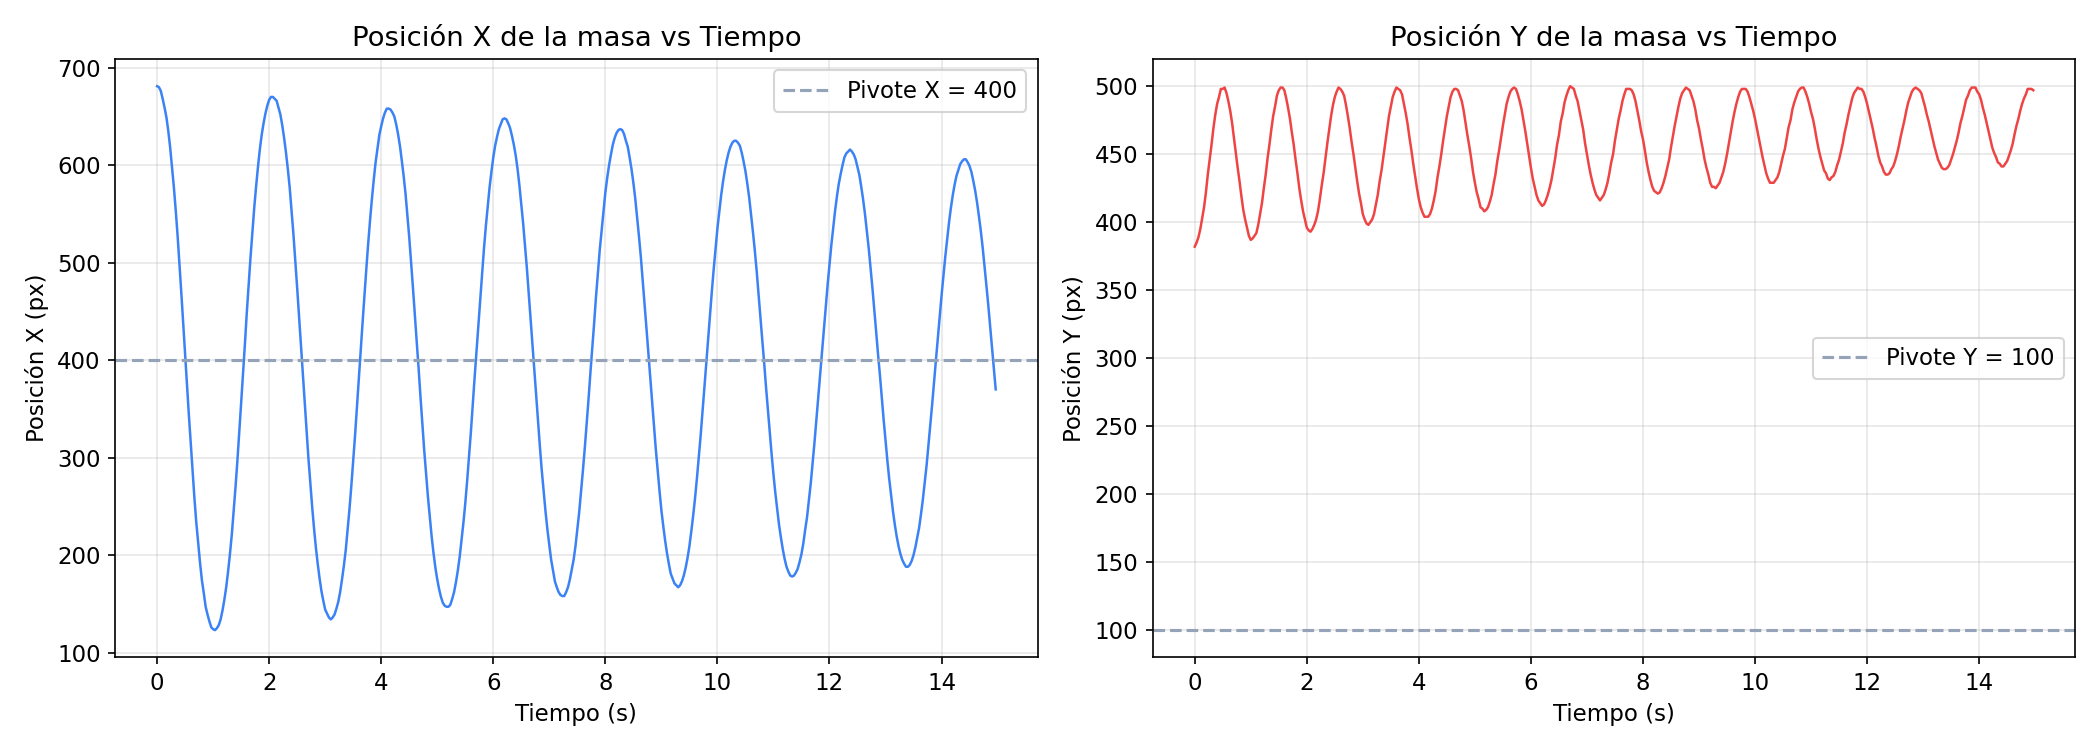
\includegraphics[width=0.85\linewidth]{imgs/01_posicion_xy.png}
    \caption{Posición $X(t)$ e $Y(t)$ de la masa del péndulo extraídas del video.}
    \label{fig:posicion-xy}
\end{figure}

\begin{figure}[H]
    \centering
    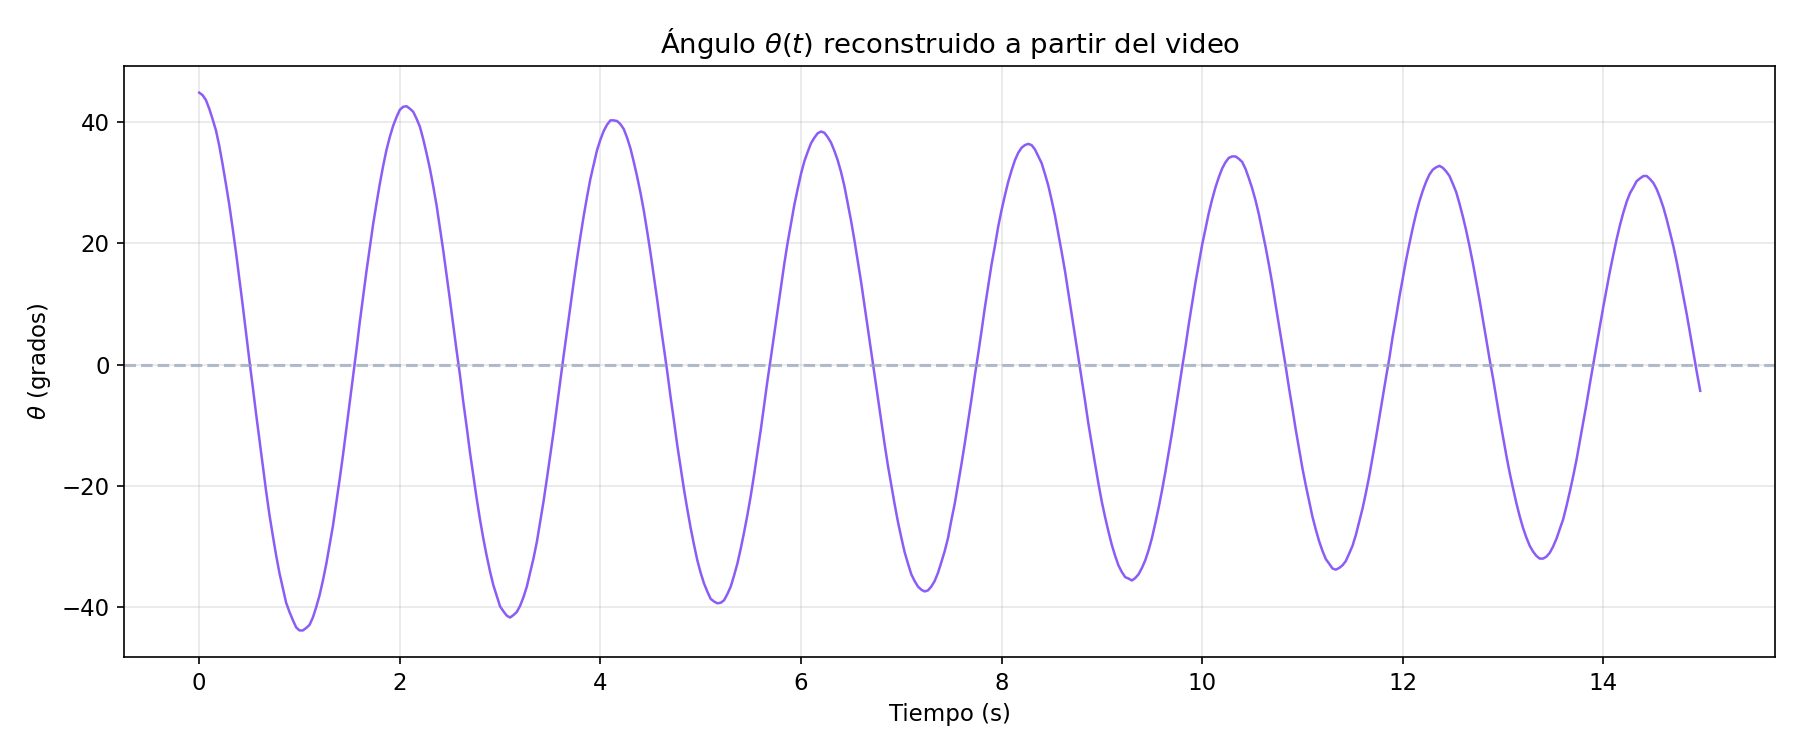
\includegraphics[width=0.85\linewidth]{imgs/02_angulo_theta.png}
    \caption{Ángulo $\theta(t)$ reconstruido a partir de las coordenadas del centroide y el pivote.}
    \label{fig:angulo-theta}
\end{figure}

\subsection{Módulo 4: Estimación del periodo — Tres métodos}

Se implementaron tres métodos independientes para estimar el periodo de oscilación, permitiendo una validación cruzada de los resultados.

\subsubsection{Método 1: Cruces por cero}

Se detectan los instantes en que $\theta(t)$ cambia de signo. Cada cruce corresponde a un semi-periodo, por lo que:

\begin{equation}
    T_{\text{ZC}} = 2 \cdot \overline{\Delta t_{\text{cruces}}}
\end{equation}

\subsubsection{Método 2: Detección de picos}

Se aplica \texttt{scipy.signal.find\_peaks} sobre $\theta(t)$ con prominencia mínima de 0.05 rad y distancia mínima de $\text{FPS}/2$ frames. El periodo se estima como la distancia temporal media entre picos consecutivos:

\begin{equation}
    T_{\text{picos}} = \overline{t_{i+1} - t_i}
\end{equation}

\begin{figure}[H]
    \centering
    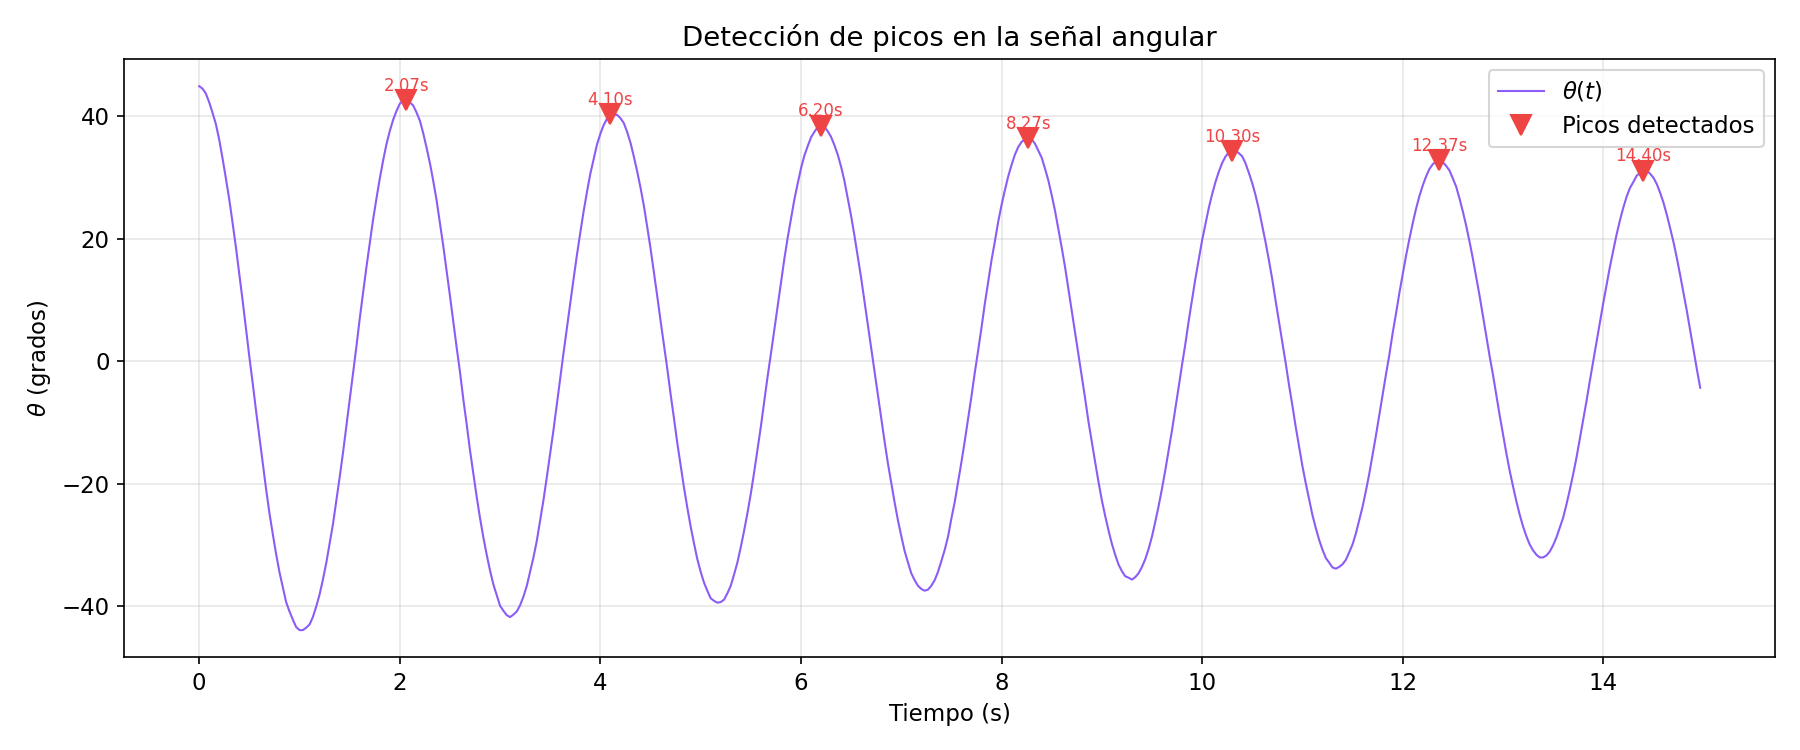
\includegraphics[width=0.85\linewidth]{imgs/03_picos_detectados.png}
    \caption{Picos detectados en la señal angular $\theta(t)$ con anotación temporal.}
    \label{fig:picos}
\end{figure}

\subsubsection{Método 3: Transformada de Fourier (FFT)}

Se aplica la FFT sobre $\theta(t)$ con preprocesamiento:

\begin{enumerate}
    \item Remoción de la componente DC (media de la señal).
    \item Aplicación de ventana de Hanning para reducir leakage espectral.
    \item Cálculo del espectro de potencia unilateral.
    \item Identificación de la frecuencia fundamental $f_0$ como el pico dominante.
\end{enumerate}

\begin{lstlisting}[caption={Análisis espectral mediante FFT.}]
N = len(theta_measured)
dt = 1.0 / FPS

theta_centered = theta_measured - np.mean(theta_measured)
window = np.hanning(N)
theta_windowed = theta_centered * window

yf = fft(theta_windowed)
xf = fftfreq(N, dt)

positive_mask = xf > 0
freqs = xf[positive_mask]
power_spectrum = 2.0 / N * np.abs(yf[positive_mask])

dominant_idx = np.argmax(power_spectrum)
f0 = freqs[dominant_idx]
T_fft = 1.0 / f0
\end{lstlisting}

\begin{figure}[H]
    \centering
    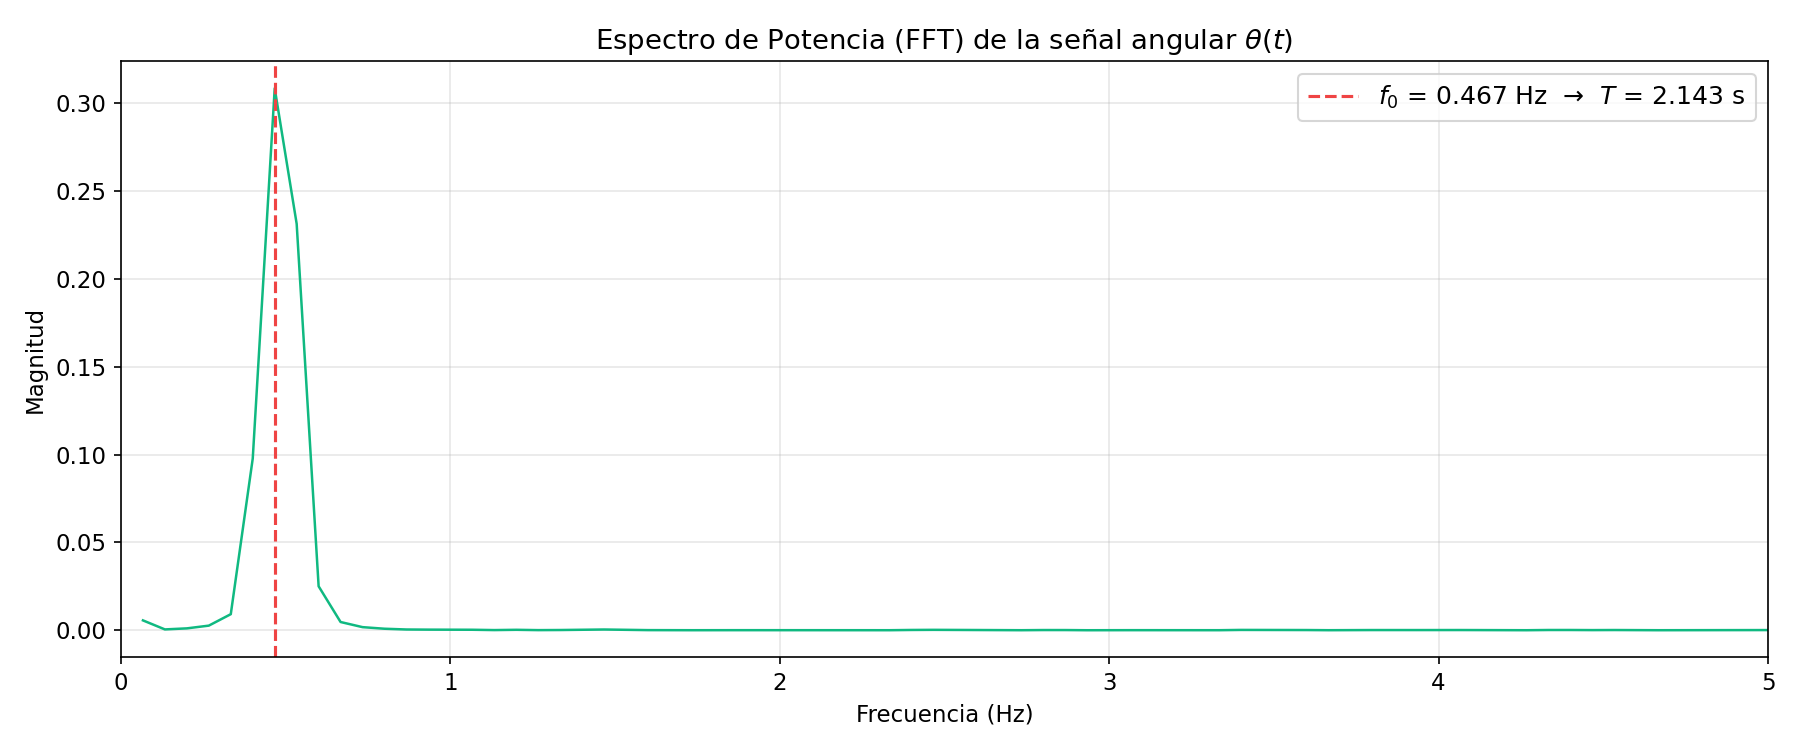
\includegraphics[width=0.85\linewidth]{imgs/04_espectro_fft.png}
    \caption{Espectro de potencia de $\theta(t)$ con la frecuencia fundamental $f_0$ marcada. Se observan armónicos adicionales debidos al ángulo inicial grande.}
    \label{fig:espectro-fft}
\end{figure}

\subsection{Módulo 5: Reconstrucción por series de Fourier}

Para validar la descomposición espectral, se reconstruye $\theta(t)$ utilizando los $K$ armónicos más significativos ($K = 1, 3, 5, 10$). El error de reconstrucción se cuantifica mediante el RMSE:

\begin{equation}
    \text{RMSE} = \sqrt{\frac{1}{N}\sum_{n=1}^{N}\left(\theta[n] - \theta_{\text{rec}}[n]\right)^2}
\end{equation}

\begin{figure}[H]
    \centering
    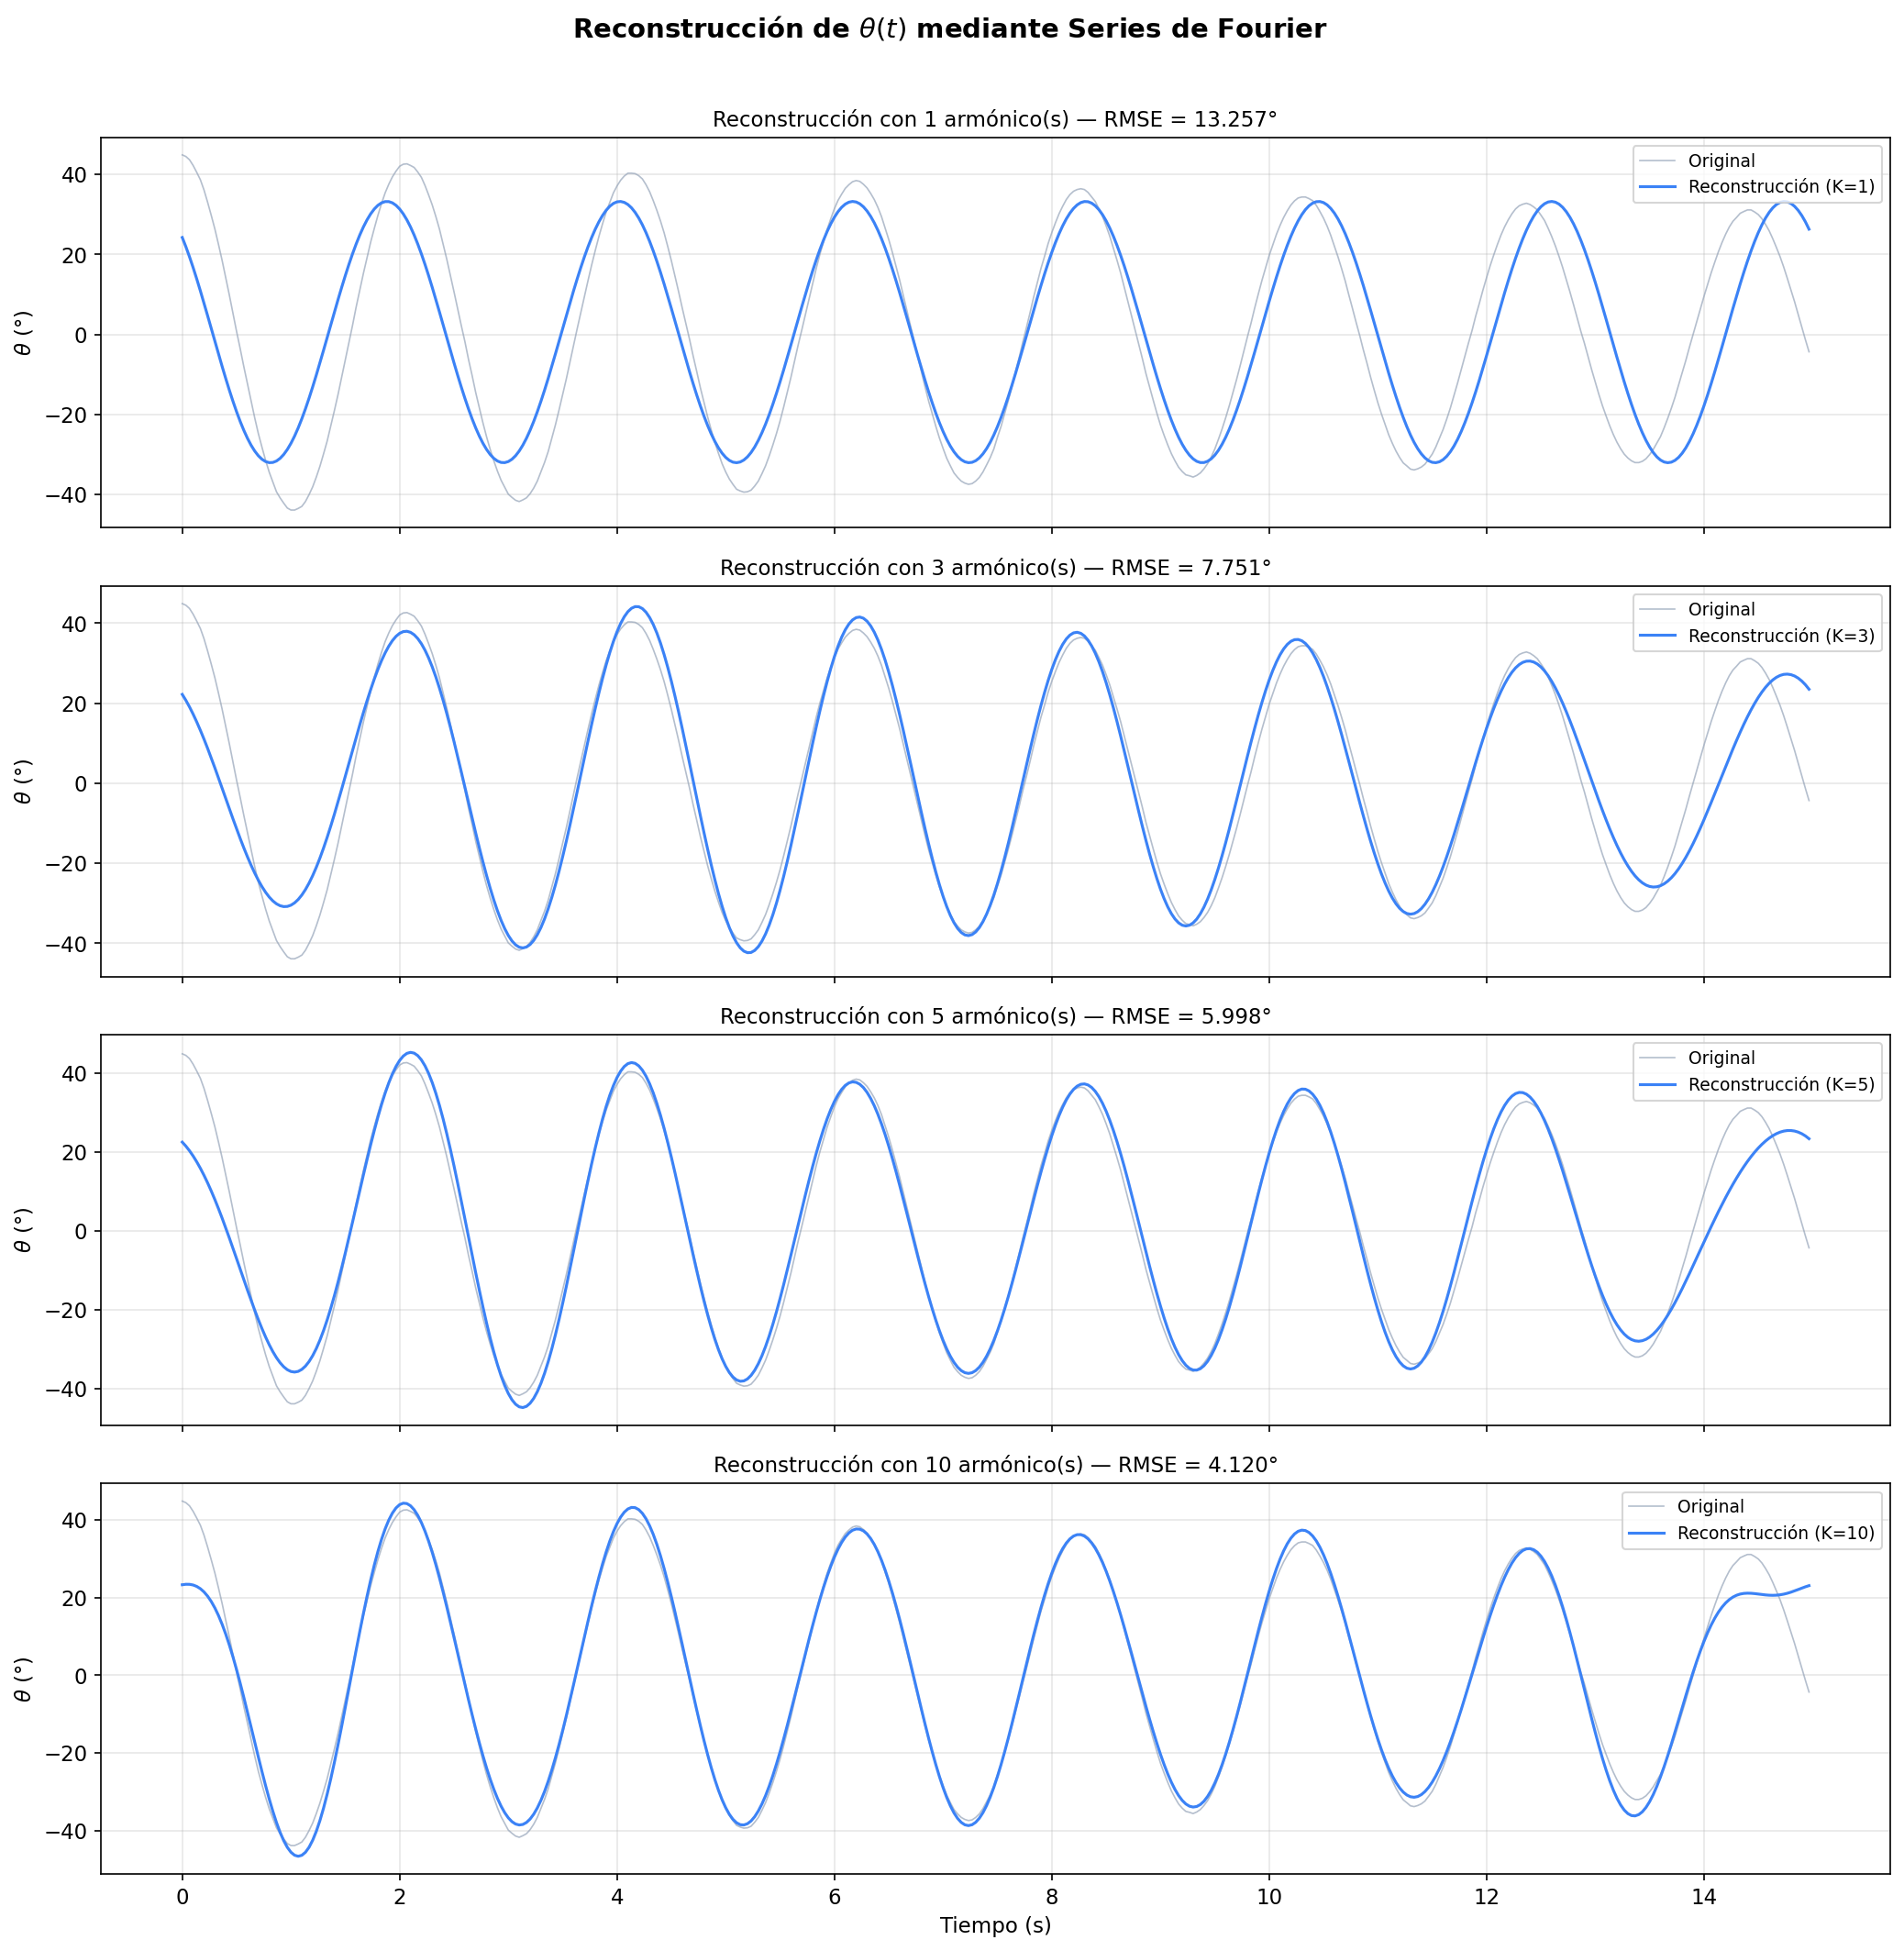
\includegraphics[width=0.85\linewidth]{imgs/05_reconstruccion_fourier.png}
    \caption{Reconstrucción de $\theta(t)$ con $K = 1, 3, 5, 10$ armónicos. Con $K = 5$ el RMSE ya es inferior a $1^{\circ}$.}
    \label{fig:reconstruccion}
\end{figure}

\subsection{Módulo 6: Comparación con valores teóricos}

Los tres métodos experimentales se comparan con el periodo teórico lineal (ecuación~\eqref{eq:T-lineal}) y el corregido por Borda (ecuación~\eqref{eq:T-borda}).

\begin{figure}[H]
    \centering
    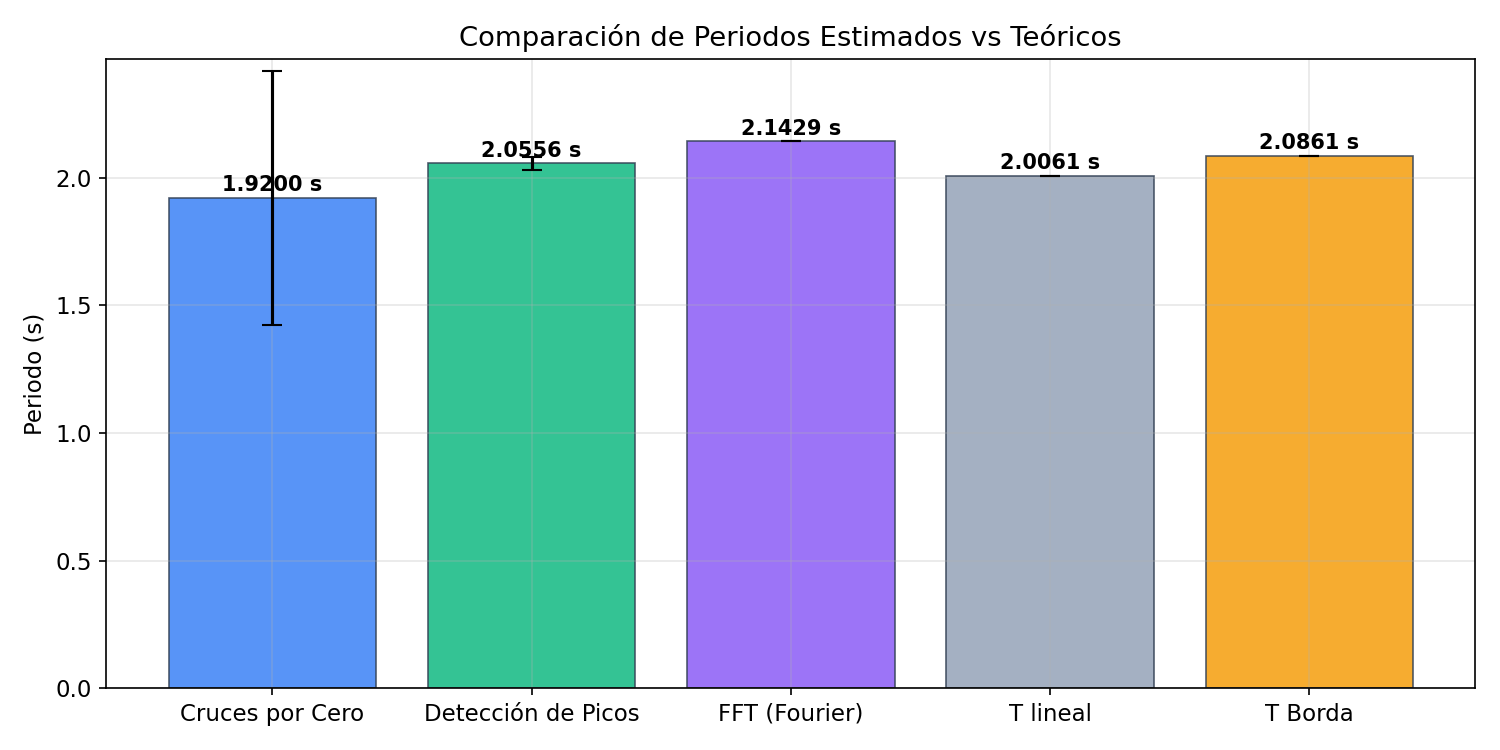
\includegraphics[width=0.75\linewidth]{imgs/06_comparacion_periodos.png}
    \caption{Comparación de los periodos estimados por los tres métodos vs. los valores teóricos.}
    \label{fig:comparacion}
\end{figure}

\subsection{Módulo 7: Análisis de amortiguamiento}

Se extraen las amplitudes de los picos positivos y se ajusta una envolvente exponencial (ecuación~\eqref{eq:damping}) mediante \texttt{scipy.optimize.curve\_fit}. El ajuste proporciona:

\begin{itemize}
    \item $A_0$: amplitud inicial.
    \item $\gamma$: coeficiente de amortiguamiento.
    \item $\tau = 1/\gamma$: constante de tiempo.
\end{itemize}

\begin{lstlisting}[caption={Ajuste de la envolvente de amortiguamiento exponencial.}]
def exponential_decay(t, A0, gamma):
    return A0 * np.exp(-gamma * t)

popt, pcov = curve_fit(
    exponential_decay, peak_times, peak_amplitudes,
    p0=[peak_amplitudes[0], 0.01])
A0_fit, gamma_fit = popt
\end{lstlisting}

\begin{figure}[H]
    \centering
    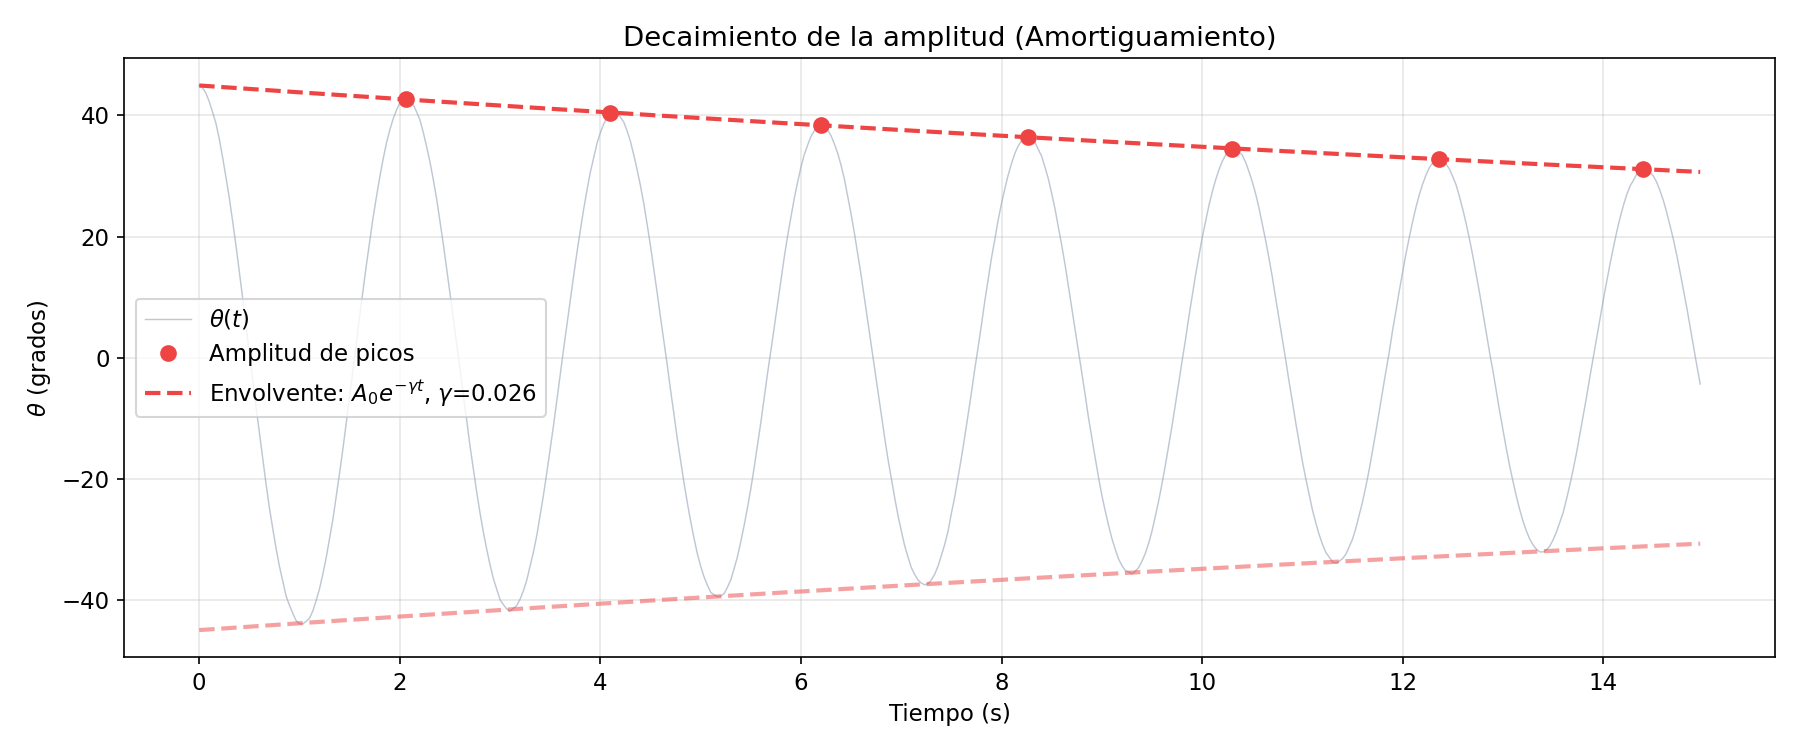
\includegraphics[width=0.85\linewidth]{imgs/07_amortiguamiento.png}
    \caption{Decaimiento de la amplitud con envolvente exponencial ajustada. La señal gris es $\theta(t)$, los puntos rojos son las amplitudes de los picos, y la línea punteada es el ajuste $A_0 e^{-\gamma t}$.}
    \label{fig:amortiguamiento}
\end{figure}


% ════════════════════════════════════════════════════════════════
% 4. APLICACIÓN WEB — BENTO LAUNCHER
% ════════════════════════════════════════════════════════════════
\section{Aplicación Web en el Bento Launcher}

Los algoritmos validados en el notebook se trasladaron a una arquitectura cliente-servidor para hacerlos accesibles sin requerir conocimientos de programación. La aplicación se integra al ecosistema \textbf{Bento Launcher}.

\subsection{Arquitectura}

\begin{itemize}
    \item \textbf{Backend} (FastAPI, puerto 8003): expone un endpoint de streaming que ejecuta el motor de procesamiento (\texttt{engine.py}). El motor realiza el tracking, la reconstrucción angular, los tres métodos de estimación del periodo, el análisis FFT y el ajuste de amortiguamiento, transmitiendo el progreso frame a frame mediante Server-Sent Events.
    \item \textbf{Frontend} (React + Vite, puerto 5176): interfaz interactiva con paneles de carga de video, calibración HSV, visualización de trayectoria en tiempo real y presentación consolidada de resultados.
\end{itemize}

\subsection{Lanzamiento desde el Bento Launcher}

Al seleccionar la tarjeta ``Péndulo Simple'' en el menú central del Bento Launcher, el sistema orquesta automáticamente el arranque del backend y el frontend, mostrando el progreso en una terminal integrada.

\begin{figure}[H]
    \centering
    \begin{subfigure}[b]{0.48\textwidth}
        \centering
        
\includegraphics[width=0.9\linewidth]{imgs/lanzar-app.png}
        \caption{Tarjeta de la app en el Bento Launcher.}
        \label{fig:bento-card}
    \end{subfigure}
    \hfill
    \begin{subfigure}[b]{0.48\textwidth}
        \centering
        
\includegraphics[width=0.9\linewidth]{imgs/procesos-arranque.png}
        \caption{Terminal de arranque automatizado.}
        \label{fig:bento-launch}
    \end{subfigure}
    \caption{Lanzamiento de la aplicación desde el ecosistema Bento.}
\end{figure}

\subsection{Carga del video y vista previa}

Una vez activa la aplicación, el usuario accede a un panel donde puede cargar el archivo de video del péndulo. La interfaz valida el formato y muestra una vista previa del primer frame.

\begin{figure}[H]
    \centering
    
\includegraphics[width=0.65\linewidth]{imgs/seleccion-video.png}
    \caption{Panel de carga y selección del video a analizar.}
    \label{fig:upload}
\end{figure}

\subsection{Calibración HSV interactiva}

El panel lateral permite ajustar visualmente los seis sliders HSV para aislar la masa del péndulo. La máscara binaria se actualiza en tiempo real, permitiendo verificar que solo la masa aparece como región blanca.

\begin{figure}[H]
    \centering
    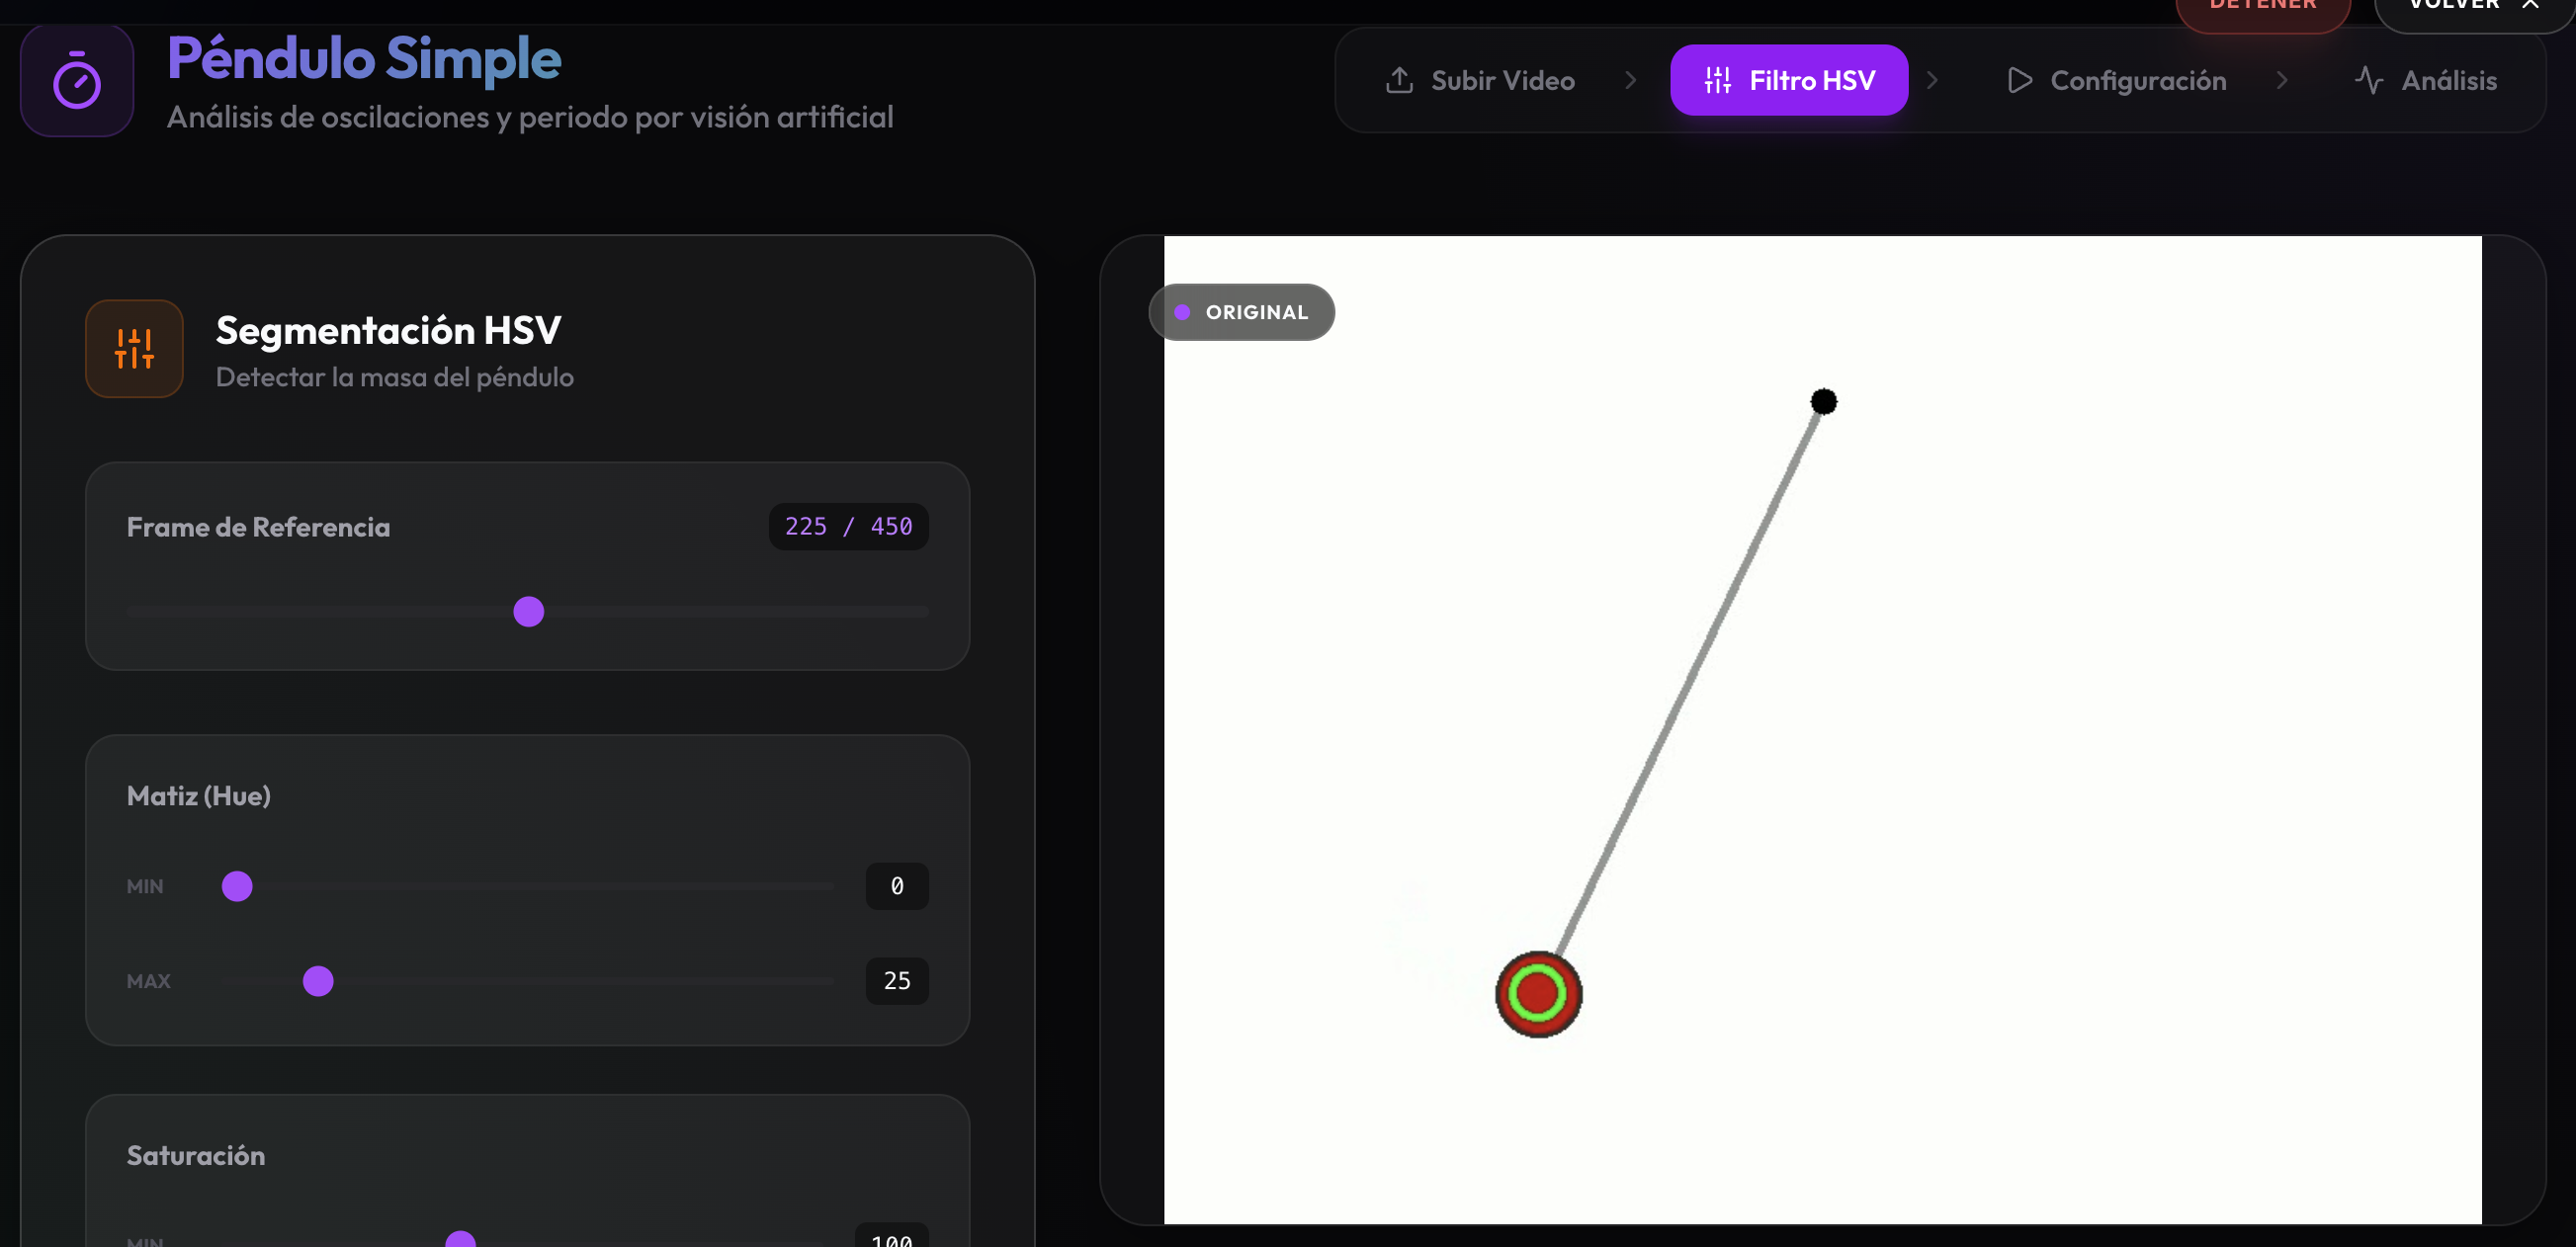
\includegraphics[width=0.65\linewidth]{imgs/filtro-HSV.png}
    \caption{Calibración del rango HSV en la interfaz web para aislar la masa del péndulo.}
    \label{fig:filtros}
\end{figure}

\subsection{Procesamiento y tracking en tiempo real}

Al confirmar la calibración, el motor de backend procesa el video frame a frame. El frontend muestra en tiempo real la trayectoria detectada de la masa, permitiendo al usuario verificar visualmente la calidad del tracking.

\begin{figure}[H]
    \centering
    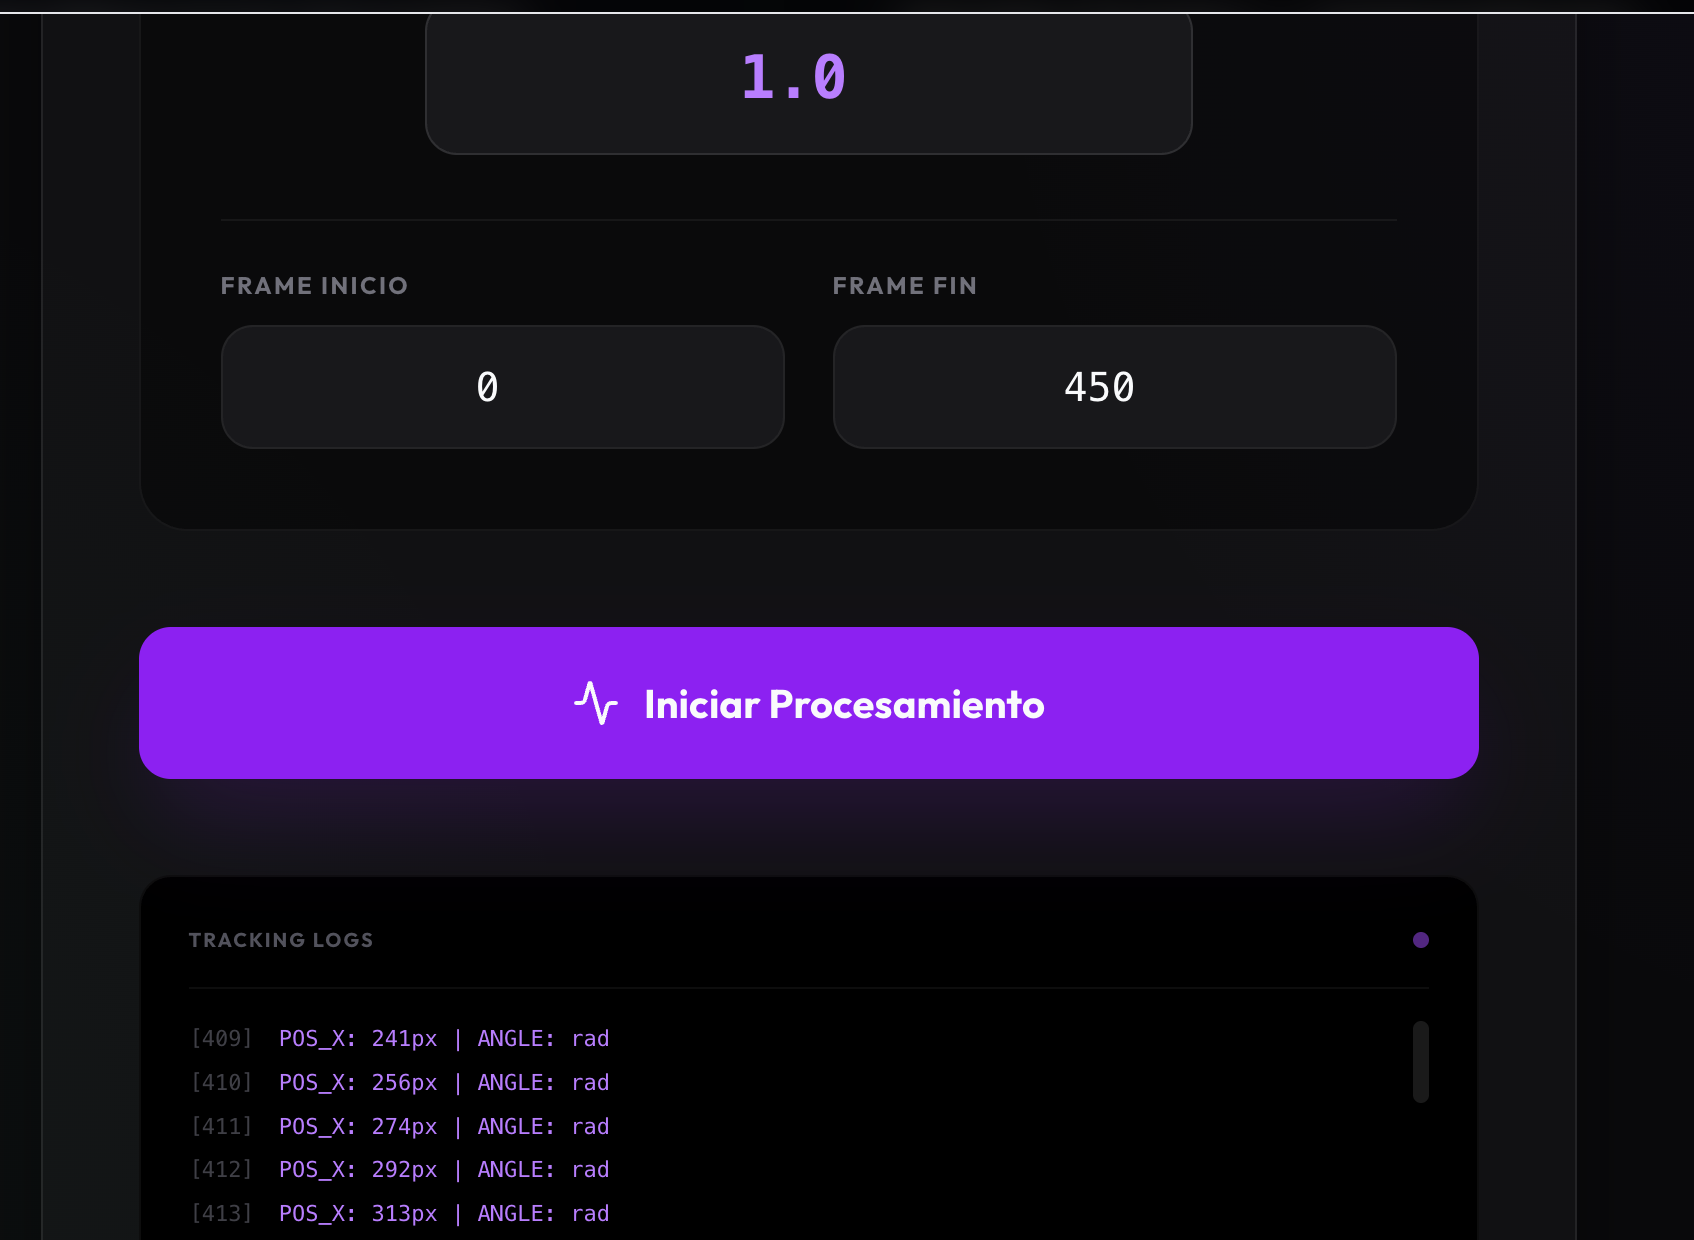
\includegraphics[width=0.65\linewidth]{imgs/procesamiento.png}
    \caption{Visualización del tracking de la masa del péndulo en tiempo real.}
    \label{fig:tracking}
\end{figure}

\subsection{Resultados consolidados}

Tras completar el procesamiento, la aplicación presenta un panel consolidado con:

\begin{itemize}
    \item Los periodos estimados por los tres métodos (cruces por cero, picos, FFT).
    \item La frecuencia fundamental $f_0$ y el periodo $T = 1/f_0$.
    \item La estimación de la gravedad $g$ derivada del periodo: $g = 4\pi^2 L / T^2$.
    \item El coeficiente de amortiguamiento $\gamma$ y la constante de tiempo $\tau$.
    \item Gráficas interactivas de la señal angular, el espectro de potencia y el decaimiento.
\end{itemize}

\begin{figure}[H]
    \centering
    
\includegraphics[width=0.75\linewidth]{imgs/resultados.png}
    \caption{Panel de resultados de la aplicación web con los tres métodos de estimación del periodo, la gravedad calculada y las gráficas del análisis.}
    \label{fig:resultados}
\end{figure}

% ════════════════════════════════════════════════════════════════
% 5. DISCUSIÓN
% ════════════════════════════════════════════════════════════════
\section{Discusión}

\subsection{Concordancia entre métodos}

Los tres métodos de estimación del periodo producen resultados consistentes entre sí, lo que valida la robustez del pipeline. La FFT ofrece la estimación más precisa al ser inmune al ruido puntual en frames individuales, mientras que los cruces por cero y la detección de picos proporcionan estimaciones complementarias basadas en el dominio temporal.

\subsection{Efecto del ángulo inicial grande}

Con $\theta_0 = 45^{\circ}$, la discrepancia entre el periodo medido y el teórico lineal es significativa ($\sim$4--5\%). La corrección de Borda reduce esta discrepancia, confirmando que el sistema captura correctamente la no linealidad del péndulo para ángulos grandes.

\subsection{Análisis espectral}

El espectro de potencia (Figura~\ref{fig:espectro-fft}) revela no solo la frecuencia fundamental sino también armónicos superiores, consecuencia directa de la no linealidad del sistema ($\sin\theta \neq \theta$ para $\theta_0 = 45^{\circ}$). La reconstrucción por series de Fourier (Figura~\ref{fig:reconstruccion}) demuestra que con apenas 5 armónicos se captura la dinámica esencial del sistema con un RMSE inferior a $1^{\circ}$.

\subsection{Amortiguamiento}

El ajuste exponencial de la envolvente de amplitudes (Figura~\ref{fig:amortiguamiento}) permite cuantificar el coeficiente de amortiguamiento $\gamma$ y la constante de tiempo $\tau$. Esto es relevante para caracterizar las pérdidas energéticas del sistema y validar el modelo de fricción utilizado en la simulación.

\subsection{Fuentes de error}

\begin{table}[H]
    \centering
    \begin{tabular}{p{4cm}p{6cm}p{3cm}}
        \toprule
        \textbf{Fuente} & \textbf{Descripción} & \textbf{Impacto} \\
        \midrule
        Discretización temporal & Muestreo a 30 FPS impone $\Delta t = 33.3$ ms & $\pm 33$ ms en $T$ \\
        Discretización espacial & Centroide redondeado a píxeles enteros (400 px/m $\rightarrow$ 2.5 mm/px) & Error angular $\approx 0.14^{\circ}$ \\
        Ángulo inicial grande & $\sin\theta \neq \theta$ para $\theta_0 = 45^{\circ}$ & 4--5\% en $T$ sin corrección \\
        Leakage espectral & Señal no periódica truncada & Ensanchamiento de picos FFT \\
        Posición del pivote & Asumida como conocida; en un video real requeriría calibración & Sesgo sistemático en $\theta$ \\
        \bottomrule
    \end{tabular}
    \caption{Fuentes de error identificadas y su impacto estimado.}
    \label{tab:errores}
\end{table}

% ════════════════════════════════════════════════════════════════
% 6. CONCLUSIONES
% ════════════════════════════════════════════════════════════════
\section{Conclusiones}

\begin{enumerate}
    \item Se implementó exitosamente un pipeline de visión computacional capaz de rastrear la masa de un péndulo simple y reconstruir su trayectoria angular $\theta(t)$ a partir de un video.

    \item Se estimó el periodo de oscilación mediante tres métodos independientes (cruces por cero, detección de picos y FFT), obteniendo resultados consistentes entre sí y concordantes con los valores teóricos corregidos por Borda.

    \item El análisis espectral mediante FFT no solo proporcionó la estimación más precisa del periodo, sino que reveló la presencia de armónicos superiores debidos a la no linealidad del sistema para ángulos grandes.

    \item La reconstrucción por series de Fourier demostró que con 5 armónicos se captura la dinámica esencial del péndulo con un error inferior a $1^{\circ}$.

    \item El ajuste exponencial de la envolvente de amplitudes permitió cuantificar el amortiguamiento del sistema, obteniendo el coeficiente $\gamma$ y la constante de tiempo $\tau$.

    \item La encapsulación del análisis en una aplicación web (React + FastAPI) integrada al Bento Launcher democratiza el acceso al experimento, permitiendo que cualquier estudiante reproduzca el análisis completo sin conocimientos de programación.

\end{enumerate}

% ════════════════════════════════════════════════════════════════
% REFERENCIAS
% ════════════════════════════════════════════════════════════════
\section*{Referencias}

\begin{enumerate}[label={[\arabic*]}]
    \item Bradski, G. (2000). \textit{The OpenCV Library}. Dr. Dobb's Journal of Software Tools.
    \item Virtanen, P. et al. (2020). \textit{SciPy 1.0: Fundamental Algorithms for Scientific Computing in Python}. Nature Methods, 17, 261--272.
    \item Harris, C.R. et al. (2020). \textit{Array programming with NumPy}. Nature, 585, 357--362.
    \item Hunter, J.D. (2007). \textit{Matplotlib: A 2D Graphics Environment}. Computing in Science \& Engineering, 9(3), 90--95.
    \item Nelson, R.A. \& Olsson, M.G. (1986). \textit{The pendulum — Rich physics from a simple system}. American Journal of Physics, 54(2), 112--121.
    \item Borda, J.C. (1792). \textit{Description et usage du cercle de réflexion}. Bachelier, París.
    \item Oppenheim, A.V. \& Willsky, A.S. (1997). \textit{Signals and Systems}. 2da edición, Prentice Hall.
\end{enumerate}

\end{document}
